% !TEX root = ../../../proposal.tex
In this section, we describe our cross-protocol DROWN attack that uses an
\ssltwo server as an oracle to efficiently decrypt TLS connections. The
attacker learns the session key for targeted TLS connections but does not
learn the server's private RSA key. We first describe our techniques using a
generic \ssltwo oracle. In Section~\ref{vulnerability}, we show how a
protocol flaw in \ssltwo can be used to construct such an oracle, and
describe our general DROWN attack. In Section~\ref{sec:special}, we show how
an implementation flaw in common versions of OpenSSL leads to a more powerful
oracle and describe our efficient special DROWN attack.

%\subsection{An efficient Bleichenbacher attack}

%\subsection{Attack scenario}
\label{sec:attack-scenario}

We consider a server accepting TLS connections from clients. The connections are established using a secure, state-of-the-art TLS version (1.0--1.2) and a \texttt{TLS\_RSA} cipher suite with a private key unknown to the attacker.

%\paragraph{Server RSA key exposed via \ssltwo.}
The same RSA public key as the TLS connections is also used for \ssltwo. For
simplicity, we will refer to the servers accepting TLS and \ssltwo
connections as the same entity.

%\paragraph{The attacker's position in the network.}
Our attacker is able to passively eavesdrop on traffic between the client and
server and record RSA-based TLS traffic.
The attacker may or may not be also required to perform active man-in-the-middle
interference, as explained below.

The attacker can expect to decrypt one out of 1,000 intercepted TLS
connections in our attack for typical parameters. This is a devastating
threat in many scenarios. For example, a decrypted TLS connection might
reveal a client's HTTP cookie or plaintext password, and an attacker would
only need to successfully decrypt a single ciphertext to compromise the
client's account. In order to collect 1,000 TLS connections, the attacker
might simply wait patiently until sufficiently many connections are recorded.
A less patient attacker might use man-in-the-middle interference, as in the
BEAST attack~\cite{beast-2011}.

\ifext
In order to collect 1,000 TLS connections, the attacker might simply wait patiently until sufficiently many connections are recorded.  If the attacker's intended victim is the \emph{server}, rather than a specific client, observing this many connections from many clients might take only a short time for an attacker who is located at a company firewall or who could perform a DNS spoofing or BGP hijacking attack to redirect traffic transparently through themselves.  If the attacker's intended victim is a \emph{particular client}, this is still feasible in many cases.  As an example, the Mozilla Thunderbird email client will check for new email messages every ten minutes by default.  A targeted user will make 1,000 connections after leaving the application running for a week.

A less patient attacker might have to resort to active man-in-the-middle techniques
in order to collect the required 1,000 TLS connections.
The attacker could embed or inject malicious JavaScript on an otherwise innocuous web site to cause the client to connect repeatedly to the victim server in a short time frame, as in the BEAST attack~\cite{beast-2011}.
The attacker may also need to trigger an error in each of the connections, in order
to prevent the handshakes from using TLS session resumption.
\fi


\subsection{A generic \ssltwo oracle}

Our attacks make use of an oracle that can be queried on a ciphertext and leaks information about the decrypted plaintext; this abstractly models the information gained from an \ssltwo server's behavior.  Our \ssltwo oracles reveal many bytes of plaintext, enabling an efficient attack.

Our cryptographic oracle $\Oracle$ has the following functionality: 
$\Oracle$ decrypts an RSA ciphertext $c$ and responds with ciphertext validity based on the decrypted message $m$.  
The ciphertext is valid only if $m$ starts with \hexb{00}{02} followed by non-null padding bytes, a delimiter byte \hex{00}, and a \texttt{master\_key} $mk_{secret}$ of correct byte length $\ell_k$.
We call such a ciphertext \textit{\sslconform}.

All of the \ssltwo padding oracles we instantiate give the attacker similar information about a \PKCSconform \ssltwo ciphertext:
\begin{equation*} 
\Oracle(c) =  
\begin{cases} 
mk_{secret} & \text{ if } c^d \bmod N = 00 || 02 || PS || 00 || mk_{secret}  \\ 
0 & \text{ otherwise.} 
\end{cases} 
\end{equation*}
That is, the oracle $\Oracle(c)$ will return the decrypted message $mk_{secret}$ if it is queried on a \PKCSconform \ssltwo ciphertext $c$ corresponding to a correctly \PKCS padded encryption of $mk_{secret}$.  The attacker then learns $\ell_k + 3$ bytes of $m = c^d \bmod N$: the first two bytes are $00 || 02$, and the last $\ell_k+1$ bytes are $00 || mk_{secret}$.  The length $\ell_k$ of $mk_{secret}$ varies based on the cipher suite used to instantiate the oracle.  For export-grade cipher suites such as \texttt{SSL\_RSA\_EXPORT\_WITH\_RC2\_CBC\_40\_MD5},
%or \texttt{SSL\_RSA\_EXPORT\_WITH\_RC4\_40\_MD5}\@,
$k$ will be 5 bytes, so the attacker learns 8 bytes of $m$.

\subsection{DROWN attack template}
\label{sec:adapted-bb-compact}
Our attacker will use an \ssltwo oracle $\Oracle$ to decrypt a TLS \texttt{ClientKeyExchange}.  
The behavior of $\Oracle$ poses two problems for the attacker. First, a TLS key exchange ciphertext decrypts to a 48-byte \pms. But since no \ssltwo cipher suites have 48-byte key strengths, this means that a valid TLS ciphertext is invalid to our oracle $\Oracle$. 
In order to apply Bleichenbacher's attack, the attacker must transform the TLS ciphertext into a valid \ssltwo key exchange message. Second, $\Oracle$ is very restrictive, since it strictly checks the length of the unpadded message. 
According to Bardou et al.~\cite{efficient-padding-oracle-2012}, Bleichenbacher's attack would require 12 million queries to such an oracle.\footnote{See Table~1 in~\cite{efficient-padding-oracle-2012}. The oracle is denoted with the term \texttt{FFF}.} 
%As each query would require an exhaustive search over $2^{40}$ values, this would make the attack significantly more costly.

Our attacker overcomes these problems by following this generic attack flow:
\begin{enumerate}
 \setcounter{enumi}{-1}
	\item The attacker collects many encrypted TLS RSA key exchange messages.
	\item The attacker converts one of the intercepted TLS ciphertexts containing a 48-byte \pms to an RSA \PKCS encoded ciphertext valid to the \ssltwo oracle $\Oracle$. \ifext We accomplish this by taking advantage of RSA ciphertext malleability and a technique of Bardou et al.~\cite{efficient-padding-oracle-2012}. \fi
	\item Once the attacker has obtained a valid \ssltwo RSA ciphertext, they can continue with a modified version of Bleichenbacher's attack, and decrypt the message after many more oracle queries.
	\item The attacker then transforms the decrypted plaintext back into the original plaintext, which is one of the collected TLS handshakes.
\end{enumerate}

We describe the algorithmic improvements we use to make each of these steps efficient below.

\subsubsection{Finding an \sslconform ciphertext}
\label{sec:trimmers}
The first step for the attacker is to transform the original TLS \texttt{ClientKeyExchange} message $c_0$ from a \tlsconform ciphertext into an \sslconform ciphertext. 
\ifext
A trivial approach would be to generate multipliers $s_i \in \{s_1,s_2,\ldots\}$, and compute ciphertexts $c_i = (c_0 {s_i}^e) \bmod N$, until one gets accepted by $\Oracle$.
However, the number of generated ciphertexts would be high, because $\Oracle$ is very restrictive; for 2048-bit RSA keys and an oracle expecting a 5-byte $mk_{secret}$ the probability that a random ciphertext becomes \sslconform is $P_{rnd} \approx (1/256)^3 * (255/256)^{249} \approx 2^{-25}$.
\fi

For this task, we rely on the concept of \emph{trimmers}, which were introduced by Bardou et al.~\cite{efficient-padding-oracle-2012}. 
Assume that the message $m_{0} = {c_0}^d \bmod N$ is divisible by a small number~$t$. In that case,  $m_{0} \cdot t^{-1} \bmod{N}$ simply equals the natural number $m_{0} / t$. 
If we choose $u \approx t$, and multiply the original message by $u \cdot t^{-1}$, the resulting number will lie near the original message: $m_0 \approx m_0 / t \cdot u$.  \ifext We shall refer to such fractions as ``small'' fractions. \fi

This method gives a good chance of generating a new \sslconform message. 
Let $c_0$ be an intercepted \tlsconform RSA ciphertext, and let $m_0 = c_0^d \bmod N$ be the \ifext corresponding \fi plaintext.  We select a multiplier $s = u/t \bmod N = u t^{-1} \bmod N$ where $u$ and $t$ are coprime, compute the value $c_1 = c_0 s^e \bmod N$, and query $\Oracle(c_1)$.  We will receive a response if $m_1 = m_0 \cdot u/t$ is \sslconform.  

As an example, let us assume a 2048-bit RSA ciphertext with $\ell_k = 5$, and consider the fraction $u = 7, t = 8$.  The probability that $c_0 \cdot u/t$ will be \sslconform is 1/7,774, so we expect to make 7,774 oracle queries before obtaining a positive response from $\Oracle$. \S\ref{sec:fraction-probability} gives more details on computing these probabilities.

\subsubsection{Shifting known plaintext bytes}
\label{sec:rotations}
Once we have obtained an \sslconform ciphertext $c_1$, the oracle has also revealed the $\ell_k+1$ least significant bytes ($mk_{secret}$ together with the delimiter byte \hex{00}) and two most significant \hexb{00}{02} bytes of the \sslconform message $m_1$.  We would like to \emph{rotate} these known bytes around to the right, so that we have a large block of contiguous known most significant bytes of plaintext.
In this section, we show that this can be accomplished by multiplying by some shift $2^{-r} \bmod N$.  In other words, given an \sslconform ciphertext $c_1 = m_1^e \bmod N$, we can efficiently generate an \sslconform ciphertext $c_2 = m_2^e \bmod N$ where $m_2 = s \cdot m_1 \cdot 2^{-r} \bmod N$ and we know several most significant bytes of $m_2$. 

Let $R = 2^{8(k+1)}$ and $B = 2^{8(\ell_m-2)}$. Abusing notation slightly, let the integer $m_1 = 2 \cdot B + PS \cdot R + mk_{secret}$ be the plaintext satisfying $m_1^e = c_1 \bmod N$.  At this stage, the $\ell_k$-byte integer $mk_{secret}$ is known and the $\ell_m-\ell_k-3$-byte integer $PS$ is not.

Let $\tilde{m_1} = 2 \cdot B + mk_{secret}$ be the known components of $m_1$, so $m_1 = \tilde{m_1} + PS \cdot R$. We can use this to compute a new plaintext for which we know many most significant bytes.  Consider the value:
\[
m_1 \cdot R^{-1} \bmod N = \tilde{m_1} \cdot R^{-1} + PS \bmod N.
\]
The value of $PS$ is unknown and consists of $\ell_m-\ell_k-3$ bytes.  This means that the known value $\tilde{m_1} \cdot R^{-1}$ shares most of its $\ell_k+3$ most significant bytes with $m_1 \cdot R^{-1}$.

Furthermore, we can iterate this process by finding a new multiplier $s$ such that $m_2 = s \cdot m_1 \cdot R^{-1} \bmod N$ is also \sslconform.  A randomly chosen $s < 2^{30}$ will work with probability $2^{-25.4}$.  We can take use the bytes we have already learned about $m_1$ to efficiently compute such an $s$ with only 678 oracle queries in expectation for a 2048-bit RSA modulus.   \S\ref{sec:rotation-details} gives more details.

\subsubsection{Adapted Bleichenbacher iteration}
\label{sec:bb-iteration}
It is feasible for all of our oracles to use the previous technique to entirely recover a plaintext message.  However, for our \ssltwo protocol oracle it is cheaper after a few iterations to continue using Bleichenbacher's original attack.  We can apply the original algorithm proposed by Bleichenbacher as described in Section~\ref{sec:bleichenbacher}\ifext, with minimal modifications\fi.

Each step obtains a message that starts with the required \hexb{00}{02} bytes after two queries in expectation.
Since we know the value of the $\ell_k+1$ least significant bytes after multiplying by any integer, we can query the oracle only on multipliers that cause the $(\ell_k+1)$st least significant byte to be zero.  However, we cannot ensure that the padding string is entirely nonzero; for a 2048-bit modulus this will hold with probability 0.37.

For a 2048-bit modulus, the total expected number of queries when using this technique to fully decrypt the plaintext is $2048 * 2 / 0.37 \approx 11,000$.


%\ifext
\begin{figure}[t]
	%\centering 
	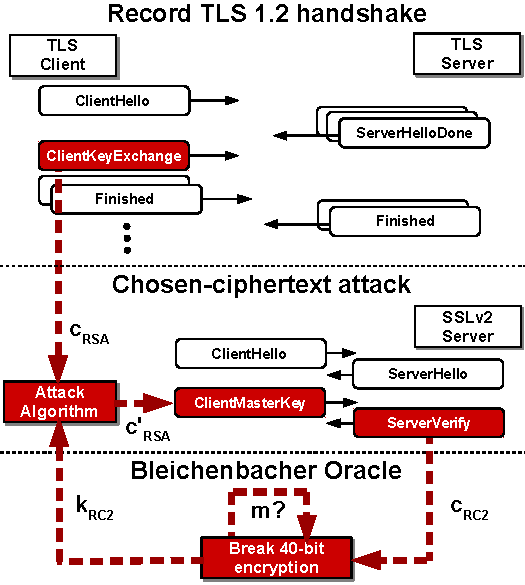
\includegraphics[width=\linewidth]{\DrownFigures/ssl-tls} 
	\caption{\textbf{\ssltwo-based Bleichenbacher attack on TLS}\,---\,%
	An attacker passively collects RSA ciphertexts from a TLS 1.2 handshake, and
    then performs oracle queries against a server that supports \ssltwo with the
	same public key to decrypt the TLS ciphertext.
	}
	\label{fig:ssl-tls}
\end{figure}
%\fi

\section{General DROWN} 
\label{vulnerability}

In this section, we describe how to use any correct \ssltwo implementation accepting export-grade cipher suites as a padding oracle.  We then show how to adapt the techniques described in Section~\ref{sec:adapted-bb-compact} to decrypt TLS RSA ciphertexts.

\subsection{The SSLv2 export padding oracle} 
\ssltwo is vulnerable to a direct message side channel vulnerability exposing a Bleichenbacher oracle to the attacker.
The vulnerability follows from three properties of \ssltwo.  First, the server immediately responds with a \texttt{ServerVerify} message after receiving the \texttt{ClientMasterKey} message, which includes the RSA ciphertext, without waiting for the \texttt{ClientFinished} message that proves the client knows the RSA plaintext.  Second, when choosing 40-bit export RC2 or RC4 as the symmetric cipher, only 5 bytes of the \texttt{master\_key} ($mk_{secret}$) are sent encrypted using RSA, and the remaining 11 bytes are sent in cleartext.  Third, a server
implementation that correctly implements the anti-Bleichenbacher countermeasure 
and receives an RSA key exchange message with invalid
padding will generate a random premaster secret and carry out the
rest of the TLS handshake using this randomly generated key material.

This allows an attacker to deduce the validity of RSA ciphertexts in the following manner:

\begin{enumerate}
	\item The attacker sends a \texttt{ClientMasterKey} message, which contains an RSA ciphertext $c_0$ and any choice of 11 clear key bytes for $mk_{clear}$. The server responds with a \texttt{ServerVerify} message, which contains the \texttt{challenge} encrypted using the \texttt{server\_write\_key}.
	\item The attacker performs an \textit{exhaustive search} over the possible values of the 5 bytes of the \texttt{master\_key} $mk_{secret}$, computes the corresponding \texttt{server\_write\_key}, and checks whether the \texttt{ServerVerify} message decrypts to \texttt{challenge}. One value should pass this check; call it $mk_0$. Recall that if the RSA plaintext was valid, $mk_0$ is the unpadded data in the RSA plaintext $c_0 ^d$. Otherwise, $mk_0$ is a randomly generated sequence of 5 bytes.
	\item The attacker re-connects to the server with the same RSA ciphertext $c_0$. The server responds with another \texttt{ServerVerify} message that contains the current \texttt{challenge} encrypted using the current \texttt{server\_write\_key}. If the decrypted RSA ciphertext was valid, the attacker can use $mk_0$ to decrypt a correct \texttt{challenge} value from the \texttt{ServerVerify} message. Otherwise, if the \texttt{ServerVerify} message does not decrypt to \texttt{challenge}, the RSA ciphertext was invalid, and $mk_0$ must have been random.
\end{enumerate}

Thus we can instantiate an oracle $\OracleSSLexp$ using the procedure above; each oracle query requires two server connections and $2^{40}$ decryption attempts in the simplest case.  For each oracle call $\OracleSSLexp(c)$, the attacker learns whether $c$ is valid, and if so, learns the two most significant bytes \hexb{00}{02}, the sixth least significant \hex{00} delimiter byte, and the value of the 5 least significant bytes of the plaintext $m$.

\ifext
If the server does not support 40-bit export ciphers, the attack can also be mounted in feasible computation time by choosing DES as the symmetric cipher.  Choosing DES means the exhaustive search is now done over a key space of 56 bits, thus increasing the cost of the attack by a factor of \begin{math} 2^{16} \end{math}, but does not fundamentally change anything except the increased cost.
\fi

\ifsubmit\relax\else
\subsection{OpenSSL special DROWN oracle}

We discovered a vulnerability present in OpenSSL versions prior to March 4, 2015 that allows a client to improperly provide cleartext key bytes for non-export ciphers.  Affected servers will substitute these bytes for bytes from the encrypted key.  This allows a client to successively learn a byte at a time of an encrypted key by brute forcing only 256 possibilities for each query. For a non-export 128-bit cipher suite such as \texttt{SSL\_RC4\_WITH\_MD5}, the attacker learns 19 bytes of the decrypted message.  We describe this vulnerability in more detail in \S~\ref{sec:clear-key-vuln}.  A client can then construct a Bleichenbacher oracle from this behavior by validating the \texttt{ServerVerify} message against the candidate key provided in the \texttt{clear\_key\_data}, resulting in no brute-force computation.
\fi

\subsection{TLS decryption attack}
\label{sec:bb-performance}

In this section, we describe how the oracle described in Section~\ref{vulnerability} can be used to carry out a feasible attack to decrypt passively collected TLS ciphertexts.

%\subsubsection{Attack scenario}
As described in Section~\ref{sec:attack-scenario}, we consider a server that accepts TLS connections from clients using an RSA public key that is exposed via \ssltwo, and an attacker who is able to passively observe these connections.

%\paragraph{Server supports export cipher suites for \ssltwo.}
We also assume the server supports export cipher suites for \ssltwo.
This can happen for two reasons.
First, the same server operators that fail to follow best practices in disabling \ssltwo~\cite{rfc6176} may also fail to follow best practices by supporting export cipher suites.
Alternatively, the server might be running a version of OpenSSL prior to January 2016, in which case it is vulnerable to the OpenSSL cipher suite selection bug described in Section~\ref{sec:openssl-selection}, and an attacker may negotiate a cipher suite of his choice independent of the server configuration.

% Nimrod: The previous subsection, introducing the generic SSLv2 oracle,
% already (implicitly) assumes this. Since we're short on space, I vote
% to remove this, at least for now.
\ifext
\paragraph{Correct Bleichenbacher countermeasure.}
We assume the server implements the recommended countermeasure against Bleichenbacher's attack in all protocol versions, including \ssltwo. If the decrypted RSA ciphertext has invalid padding, the server generates a random \pms or \texttt{master\_key} and continues the handshake with this random string. We assume this countermeasure is implemented correctly and the server is neither vulnerable to timing nor flush-and-reload side-channel attacks~\cite{Meyer14,zhang-2014}.
\fi

%\paragraph{Computing power.}
The attacker needs access to computing power sufficient to perform a $2^{50}$ time attack, mostly brute forcing symmetric key encryption.  After our optimizations, this can be done with a one-time investment of a few thousand dollars of GPUs, or in a few hours for a few hundred dollars in the cloud.  Our cost estimates are described in~Section~\ref{sec:ec2_results}.

\if0
In our simplest attack scenario, an attacker is passively observing many connections between modern clients and server who negotiate a secure TLS version (1.0--1.2) with an RSA cipher suite and a well-generated, secure RSA public key.   The server is also configured to support \ssltwo with the same certificate as in TLS if a client requests it, although the modern victim clients will never negotiate \ssltwo.  The server implements the recommended countermeasures against Bleichenbacher attacks described in Section~\ref{sec:bleichenbacher}.



Our attacker will use our SSLv2 oracle $\OracleSSL$ to decrypt a TLS \texttt{ClientKeyExchange}.  We specialize the discussion below to our protocol-level oracle described in Section~\ref{vulnerability} and refer to this attack as the \emph{general} DROWN attack.  The adaptations to the OpenSSL clear-key oracle, which produces our faster \emph{special} DROWN attack are similar and are described in Section~\ref{sec:special}.
\fi

\subsubsection{Constructing the attack}

The attacker can exploit the \ssltwo vulnerability
\ifext as illustrated in Figure~\ref{fig:ssl-tls}, \fi
following the generic attack outline described in Section~\ref{sec:adapted-bb-compact},
consisting of several distinct phases:

\begin{enumerate}
 \setcounter{enumi}{-1}
	\item The attacker passively collects 1,000 TLS handshakes from
	connections using RSA key exchange.

	\item They then attempt to convert the intercepted TLS ciphertexts containing a 48-byte \pms to valid RSA \PKCS encoded ciphertexts containing five-byte messages using the fractional trimmers described in Section~\ref{sec:trimmers}, and querying $\OracleSSLexp$. The attacker sends the modified ciphertexts to the server using fresh \ssltwo connections with weak symmetric ciphers and uses the \texttt{ServerVerify} messages to deduce ciphertext validity as described in the previous section. For each queried RSA ciphertext, the attacker must perform a brute force attack on the weak symmetric cipher. The attacker expects to obtain a valid \ssltwo ciphertext after roughly 10,000 oracle queries, or 20,000 connections to the server.

	\item Once the attacker has obtained a valid \ssltwo RSA ciphertext
	$c_1 = m_1^e$, they use the shifting technique explained in
	Section~\ref{sec:rotations} to find an integer $s_1$ such that
	$m_2 = m_1 \cdot 2^{-40} \cdot s_1$ is also \sslconform.
	\S~\ref{sec:general-rotations} contains more details on this step.

	\item The attacker then applies the shifting technique again to find
	another integer $s_2$ such that $m_3 = m_2 \cdot 2^{-40} \cdot s_2$
	is also \sslconform.

	\item They then search for yet another integer $s_3$ such that
	$m_3 \cdot s_3$ is also \sslconform.

	\item Finally, the attacker can continue with our adapted Bleichenbacher
	iteration technique described in Section~\ref{sec:bb-iteration}, and
	decrypts the message after an expected 10,000 additional oracle queries,
	or 20,000 connections to the server.

	\item The attacker can then transform the decrypted plaintext back into
	the original plaintext, which is one of the 1,000 intercepted TLS 		handshakes.

\end{enumerate}

\paragraph{The rationale behind the different phases.}
Bleichenbacher's original algorithm requires a conformant message $m_0$, and a multiplier $s_1$ such that $m_1 = m_0 \cdot s_1$ is also conformant.
Na\"{\i}vely, it would appear we can apply the same algorithm here, after completing Phase 1.
However, the original algorithm expects $s_1$ to be of size about $2^{24}$. This is not the case when we use fractions for $s_1$, as the integer $s_1 = u t^{-1} \bmod N$ will be the same size as $N$.

Therefore, our approach is to find a conformant message for which we know the 5 most significant bytes; this will happen after multiple rotations and
this message will be $m_3$.
After finding such a message, finding $s_3$ such that $m_4 = m_3 \cdot s_3$ is also conformant becomes trivial.
From there, we can finally apply the adapted Bleichenbacher iteration technique as described in \S\ref{sec:general-bleichenbacher}.

\begin{table}[t]
  \centering
	\begin{tabularx}{\linewidth}{Xrrrrr}
	\toprule
	\textbf{Optimizing For} & \textbf{Ciphertexts} & \textbf{$|F|$}     & \textbf{\ssltwo Connections}  & \textbf{Offline Work} \\
	\midrule
	offline work        &           12,743 &          1 &            50,421  & $2^{49.64}$ \\
        offline work        &            1,055 &         10 &              46,042  & $2^{50.63}$ \\
	% compromise is achieved by using fractions {8/7, 8/9}; numbers are now final
       	compromise          &            4,036 &          2 &              41,081  & $2^{49.98}$ \\
	online work         &            2,321 &          3 &              38,866  & $2^{51.99}$ \\
	online work         &              906 &          8 &              39,437  & $2^{52.25}$ \\
	\bottomrule
	\end{tabularx}
		\caption{\textbf{2048-bit Bleichenbacher attack complexity}\,---\,%
		The cost to decrypt one ciphertext can be adjusted by choosing the set of
        fractions $F$ the attacker applies to each of the passively collected
		ciphertexts in the first step of the attack. This choice affects several
		parameters: the number of these collected ciphertexts, the number of
 		connections the attacker makes to the \ssltwo server, and the number of
		offline decryption operations.
		}
        \label{tab:reasonable_parameters}
\end{table}

\begin{table}[t]
\begin{tabularx}{\linewidth}{Xrrrr}
\toprule
\textbf{Key size}    & \textbf{Phase 1} & \textbf{Phases 2--5} & \textbf{Total Queries}   & \textbf{Offline Work} \\
\midrule
% This is all when using 4/5, which has a maximal "native probability" of 0.1.
% Offline work is always step1 * 2**38
%              1024 &  (0.1 * 0.62 * 1/256)**(-1)  & + 256 / 0.62 * 2 + 2/0.62 + 1024 * 2 / 0.62
               1024 &  4,129   &  4,132  &  8,261 & $2^{50.01}$ \\

%              2048 & (0.1 * 0.37 * 1/256)**(-1)   & + (2.72 * 2**8) * 2 + 2.72*2 + 2048 * 2 / 0.37 (number for phase 5 also matches runs)
               2048 &  6,919   &  12,468 & 19,387 & $2^{50.76}$ \\

%              4096 & (0.1 * 0.14 * 1/256)**(-1)   & + 2**8 / 0.14 * 2 + 2/0.14 + 4096 * 2 / 0.14
               4096 &  18,286  &  62,185 & 80,471 & $2^{52.16}$ \\
\bottomrule
\end{tabularx}
	\caption{\textbf{Required oracle queries}\,---\,%
	In Phase 1, the attacker queries the oracle until an \ssltwo conformant
	ciphertext is found. In Phases 2--5, the attacker decrypts this ciphertext
	using leaked plaintext. These numbers minimize total queries. In our attack,
	an oracle query represents two server connections.
	}
	\label{tab:optimal_queries}
\end{table}

\newcommand{\GPUTable}{
\begin{table*}[t]
 \centering
 \begin{tabular}{llrrrr}
        \toprule
        \textbf{Platform} & \textbf{Hardware} & \textbf{Cost} & \textbf{Full attack}  & \textbf{Cost to perform attack in 1 day} \\
        \midrule
        Na\"{\i}ve CPU & 4 Intel Xeon E7-4820 & $\$21,400$ & $114$ days  & \$$2,440,000$\\
        Na\"{\i}ve GPU & ZOTAC GeForce GTX TITAN & $\$2,400$  & $189$ days & \$$450,000$ \\
        Na\"{\i}ve FPGA & 64 Spartan-6 LX150 & $\$60,000$ & $51.5$ days  & \$$3,090,000$  \\
        \cmidrule{1-5}
        Optimized Hashcat & NVIDIA GTX / AMD R9 & \$18,040 & $0.75$ days & \$13,500 \\
        Optimized EC2 & NVIDIA & \$440 & $0.33$ days & \$147 \\
        \bottomrule
    \end{tabular}	
	\caption{\textbf{Time and cost efficiency of our attack on different hardware platforms.}\,---\,%
	The brute force attacks against symmetric export keys are the most expensive
	part of our attack. We compared the performance of a na\"{\i}ve
	implementation of our attack on different platforms, and decided that a GPU
	implementation held the most promise. We then heavily optimized our GPU
	implementation, obtaining several orders of magnitude in speedup.
	}
\label{perf_comparison}
\end{table*}
}

\subsubsection{Attack performance}
The attacker wishes to minimize three major costs in the attack: the number of recorded ciphertexts from the victim client, the number of connections to the victim server, and the number of symmetric keys to be brute forced.
The requirements for each of these elements are governed by the set of fractions to be multiplied with each RSA ciphertext in the first phase, as described in Section~\ref{sec:trimmers}.

Table~\ref{tab:reasonable_parameters} highlights a few choices for $F$ and the resulting performance metrics for 2048-bit RSA keys.
Appendix \ref{sec:adapted-bb} provides more details on the derivation of these numbers and other optimization choices.
Table \ref{tab:optimal_queries} gives the expected number of Bleichenbacher queries for different RSA key sizes, when minimizing total oracle queries.

%These are fractions of small coprime numbers, similar to the example $u/t = 8/7$, and ideally amenable to the additional optimization described above.





%The special DROWN attack requires similar numbers of ciphertexts and oracle queries, but the amount of computation is negligible.


